\section{Testkonzept}\label{sec:testkonzept}

\subsection{Aufbau} \label{subsec:prinzip}

In der Abbildung \ref{fig:Testprotokoll} ist ein Überblick der Tests im Testprotokoll aufgeführt. Die detaillierten Testprotokolle, die für die internen und externen Test verwendet werden, sind im Anhang hinterlegt.

%Zur Vereinfachung als ein Bild gesehen.
\begin{figure}[H]
	\centering
	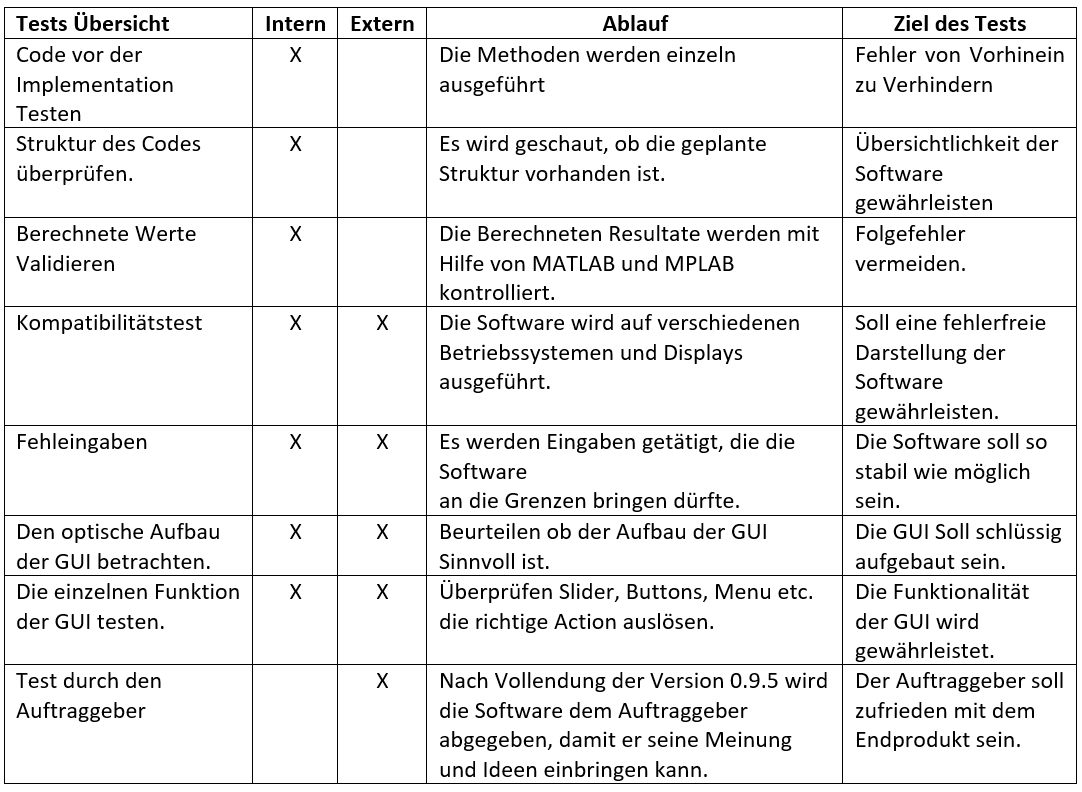
\includegraphics[width=16cm]{ueberblickTestKonzept.png}
\end{figure}

\begin{figure}[H]
	\centering
	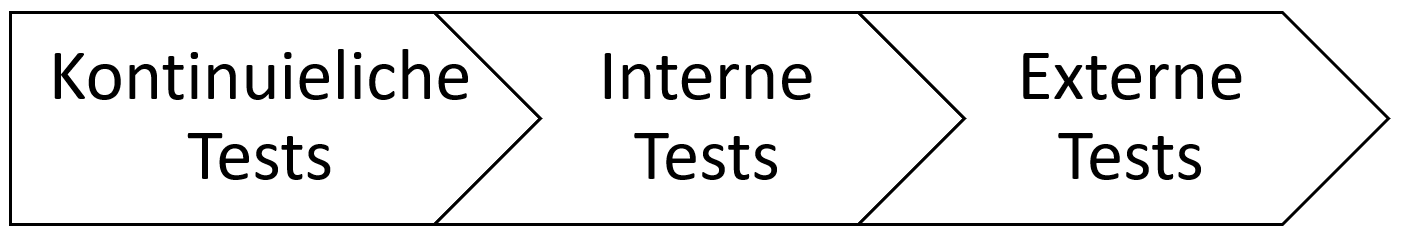
\includegraphics[width=16cm]{AblaufTestkonzept.png}
	\caption{Übersicht Testprotokoll}
	\label{fig:Testprotokoll}
\end{figure}

\newpage

\subsection{Validierung} \label{subsec:validierung}

Um sicherzustellen, dass die Simulationen richtig sind und auch korrekt dargestellt werden, werden die Ergebnisse mit entsprechenden Simulationen der Simulationssoftware MPLAB mindi verglichen. Abbildung \ref{fig:verifCM_Schema} zeigt die simulierte Gleichtaktschaltung in MPLAB mindi.

\begin{figure}[H]
	\centering
	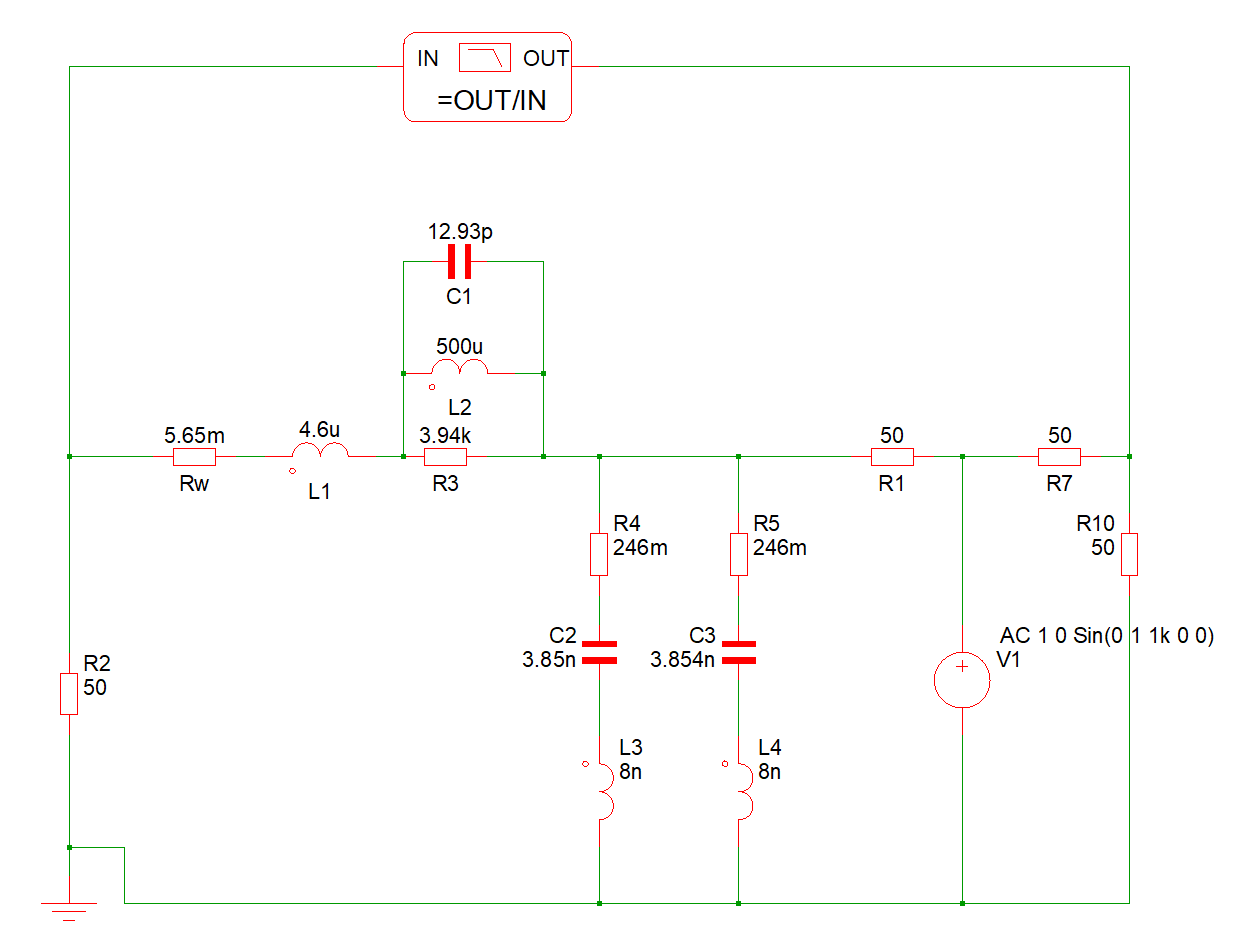
\includegraphics[width=16cm]{verifCM_Schema.png}
	\caption{Simulationsschaltung der Gleichtaktschaltung in MPLAB mindi}
	\label{fig:verifCM_Schema}
\end{figure}

Abbildung \ref{fig:verifCM_MPLAB} zeigt die Simulationsergebnisse in MPLAB mindi, welche optisch identisch sind mit den Messresultaten der entwickelten Simulationssoftware (Abbildung \ref{fig:verifCM_SW}).
 
 \begin{figure}[H]
	\centering
	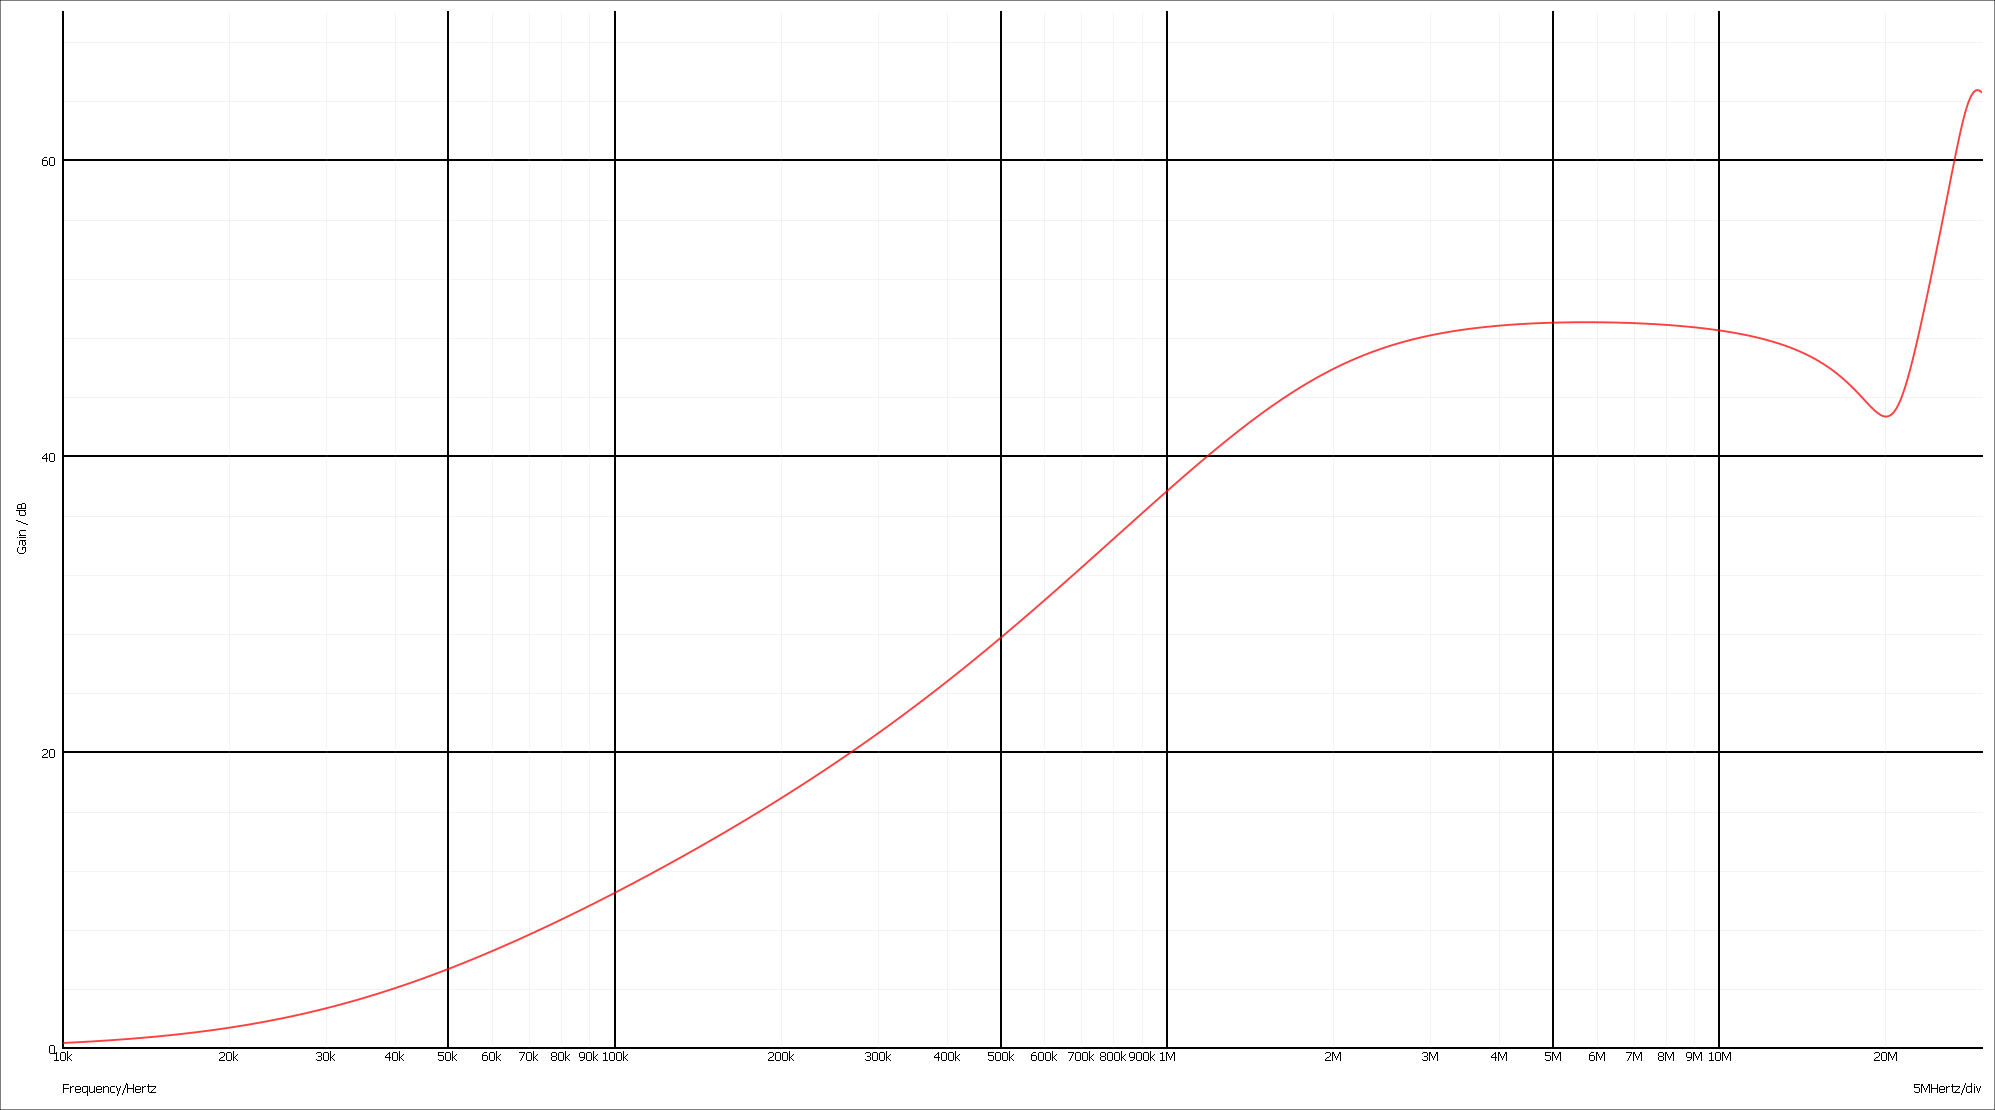
\includegraphics[width=16cm]{verifCM_MPLAB.png}
	\caption{Simulationsergebnisse der Gleichtaktschaltung in MPLAB mindi}
	\label{fig:verifCM_MPLAB}
\end{figure}

\begin{figure}[H]
	\centering
	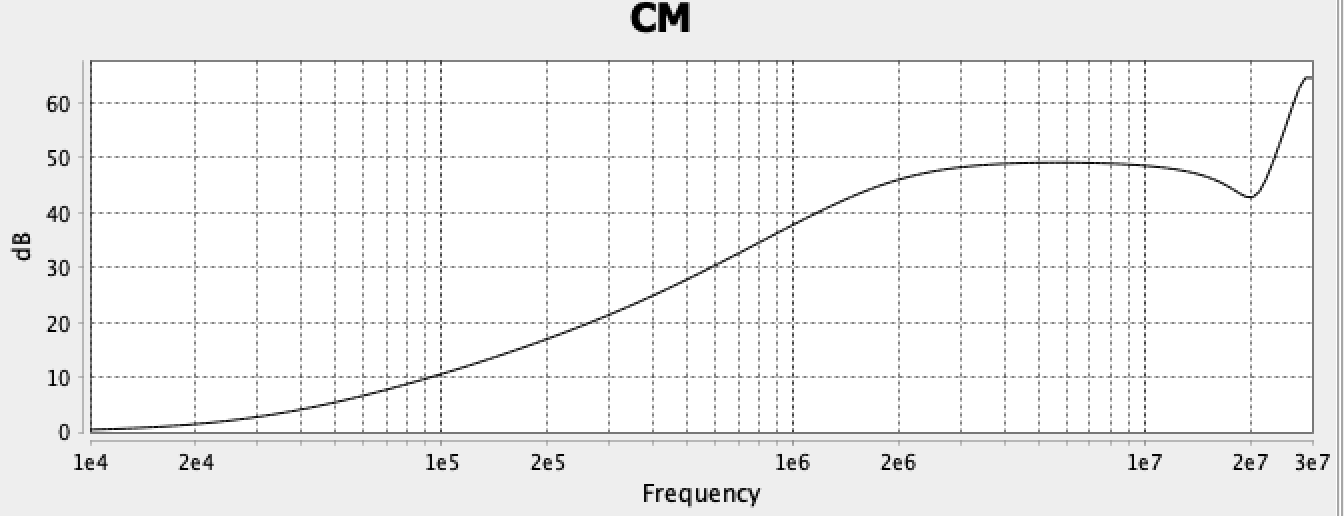
\includegraphics[width=16cm]{verifCM_SW.png}
	\caption{Simulationsergebnisse der Gleichtaktschaltung in der EMI-Filter Simulationssoftware}
	\label{fig:verifCM_SW}
\end{figure}

\newpage

Die Abbildung \ref{fig:verifDM_Schema}zeigt die simulierte Gegentaktschaltung. Die Grafik \ref{fig:verifDM_MPLAB} zeigt die daraus resultierenden Simulationen.

\begin{figure}[H]
	\centering
	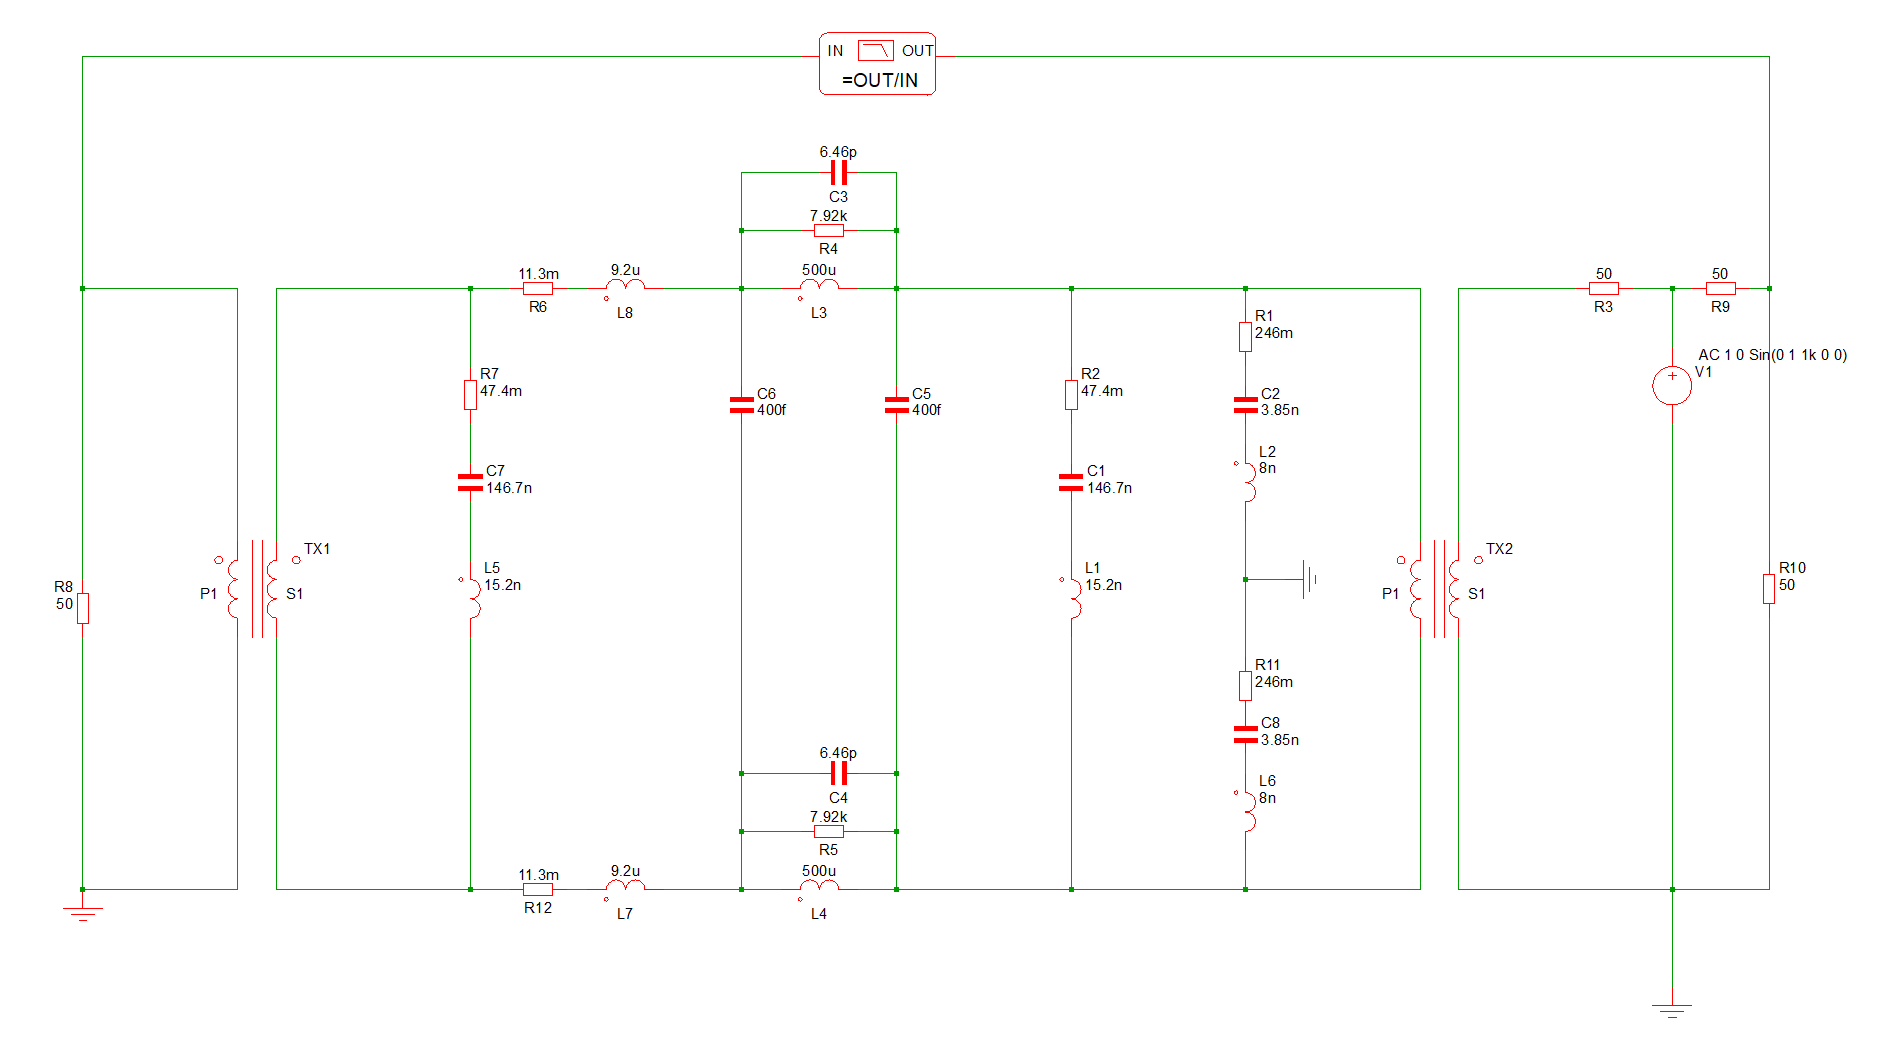
\includegraphics[width=16cm]{verifDM_Schema.png}
	\caption{Simulationsschaltung der Gegentaktschaltung in MPLAB mindi}
	\label{fig:verifDM_Schema}
\end{figure}

\newpage

\begin{figure}[H]
	\centering
	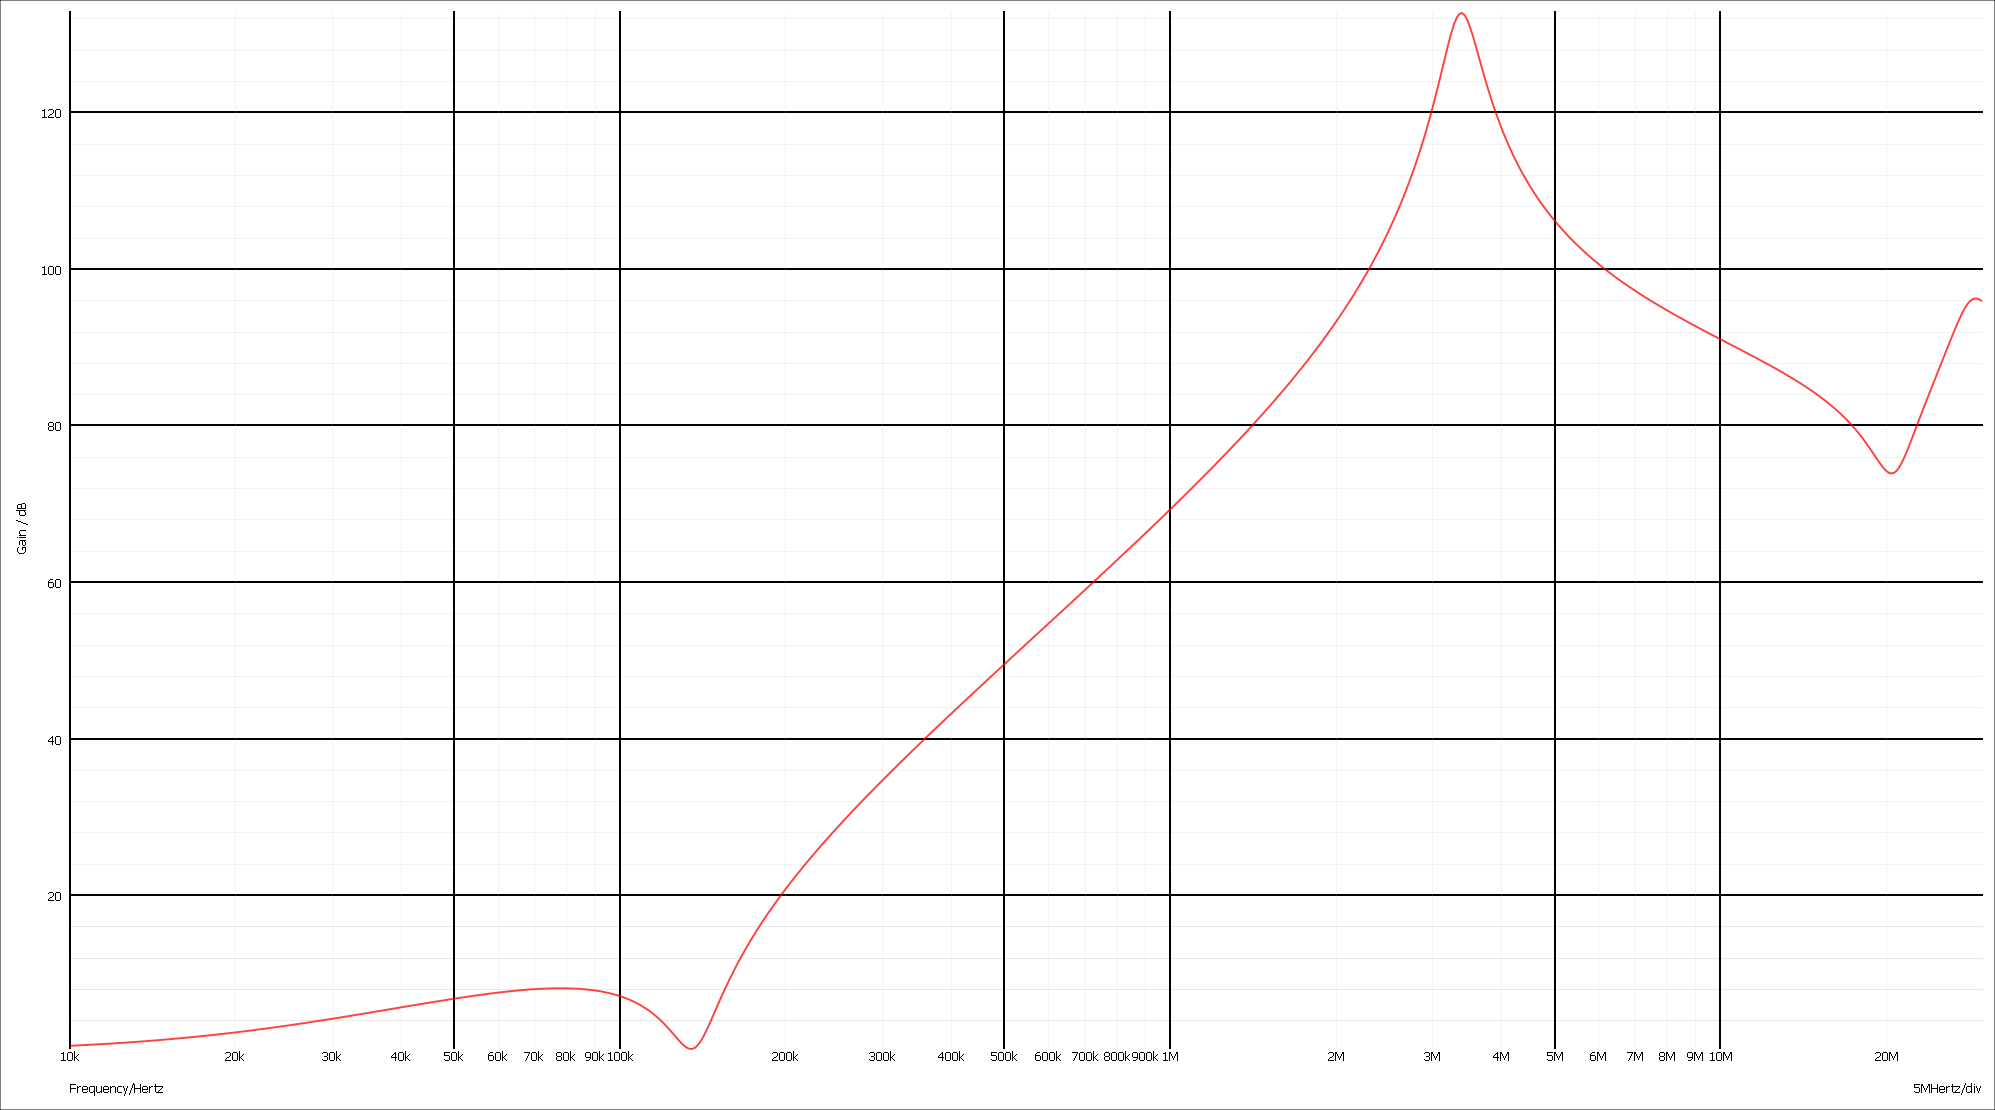
\includegraphics[width=16cm]{verifDM_MPLAB.png}
 	\caption{Simulationsergebnisse der Gegentaktschaltung in MPLAB mindi}
	\label{fig:verifDM_MPLAB}
\end{figure}

Die Ergebnisse von MPLAB mindi decken sich wiederum mit den Messresultate der entwickelten Simulationssoftware. Abbildung \ref{fig:verifDM_SW} zeigt die Resultate der entwickelten Simulationssoftware.

\begin{figure}[H]
	\centering
	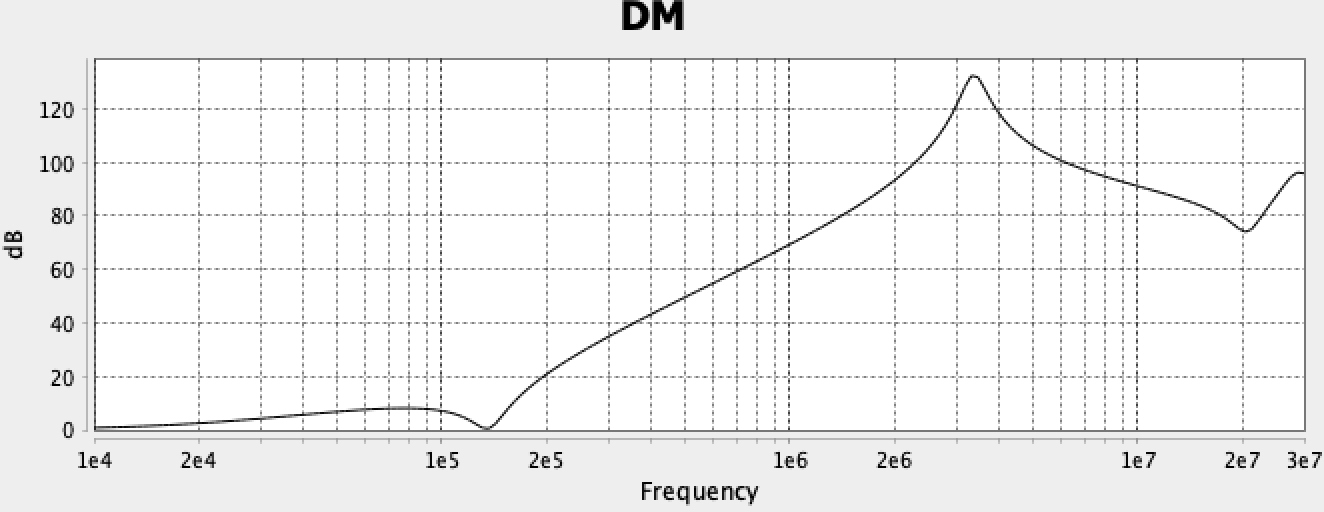
\includegraphics[width=16cm]{verifDM_SW.png}
	\caption{Simulationsergebnisse der Gegentaktschaltung in der EMI-Filter Simulationssoftware}
	\label{fig:verifDM_SW}
\end{figure}

Aus den oben beschriebenen Vergleichen wird geschlossen, dass die Berechnungen korrekt in die Software implementiert wurden.

\newpage

\subsection{Erwartungen} \label{subsec:validierung}

Die Testresultate variieren stark mit der jeweiligen Testperson, welche die Software testet.
Die internen Tests werden die groben Fehler herausfiltern und schaffen eine stabile Grundlage auf die aufgebaut werden kann. Zudem wird überprüft, ob die alle Ziele erreicht wurden.
Bei den Fachpersonen wird das Feedback höchst wahrscheinlich sehr umfangreich   ausfallen. Es ist zu erwarten, dass Fehler entdeckt werden, die noch nicht bekannt sind oder die Software gar zum Absturz gebracht wird. 
Die Fachfremden Tester werden dies nicht erreichen, jedoch erhalten wir eine Hilfreiche Rückmeldung, was die Benutzerfreundlichkeit betrifft, weil diese Personen einen anderen Blick auf das grosse ganze haben. 
Das Feedback des Auftraggebers wird sehr detailliert ausfallen, weil er genaue Vorstellungen hat was er von dem Produkt haben möchte. Es wird sich, aber vermutlich mehrheitlich, um die Funktionen drehen und nicht welche Fehler es gibt. 





